\newpage
\section{Rete per uno Stabilimento Balneare}%
\label{sec:rete}

Ci viene chiesto di progettare una rete LAN per uno stabilimento balneare. Ho progettato la rete con Cisco Packet Tracer utilizzando la versione 8.0--2, la topologia della rete \`e inclusa in questo documento nella sotto-sezione~\ref{sub:topologia}.

Ho scelto di dividere la rete dello Stabilimento Balneare in due sottoreti. La prima, che ho chiamato \emph{LAN Amministrazione}, contiene la rete utilizzata dai dipendenti con completo accesso a Internet e il server DHCP che assegna gli indirizzi IP dell'intera rete. La seconda sottorete l'ho dedicata alla rete Wireless. Ho ipotizzato che lo stabilimento balneare in questione offrisse l'accesso Wi-Fi gratuito per buona parte della spiaggia oltre che nel ristorante quindi ho anche previsto l'installazione di \emph{Access Point} per l'esterno in parte dello Stabilimento.

Nella parte a sinistra della Topologia ho simulato la rete Internet con un paio di server installati nello spazio di indirizzi IP pubblici. Il router di bordo dell'ISP mette in comunicazione la rete Internet con la rete private dello Stabilimento.

Per simulare una rete reale ho configurato la rete dello Stabilimento per utilizzare il NAT/PAT\@: le richieste vengono modificate dal Router centrale e viene sostituito l'indirizzo IP sorgente con l'indirizzo del Router, il Router poi invia il pacchetto utilizzando una porta casuale in uscita e associa la porta utilizzata all'indirizzo IP del vero dispositivo sorgente, quando riceve risposte con destinazione quella porta, modifica nuovamente il pacchetto ma questa volta sostituisce l'indirizzo di destinazione da quello del router a quello del dispositivo all'interno della rete e lo invia il pacchetto verso di esso. Questo procedimento permette di utilizzare gli indirizzi privati per comunicare con la rete Internet senza richiedere un indirizzo IP pubblico per ogni dispositivo, all'esterno comparir\`a l'indirizzo IP pubblico della rete come sorgente.

La rete pubblica deve essere monitorata e informazioni sul traffico e sull'individuo che l'ha originato devono essere salvate all'interno di file di log. A causa delle limitazioni di Cisco Packet Tracer non \`e stato possibile implementare il login hotspot all'interno della rete tuttavia in una situazione reale \`e necessario.

\begin{landscape}
    \subsection{Topologia}%
    \label{sub:topologia}
    \thispagestyle{empty}
    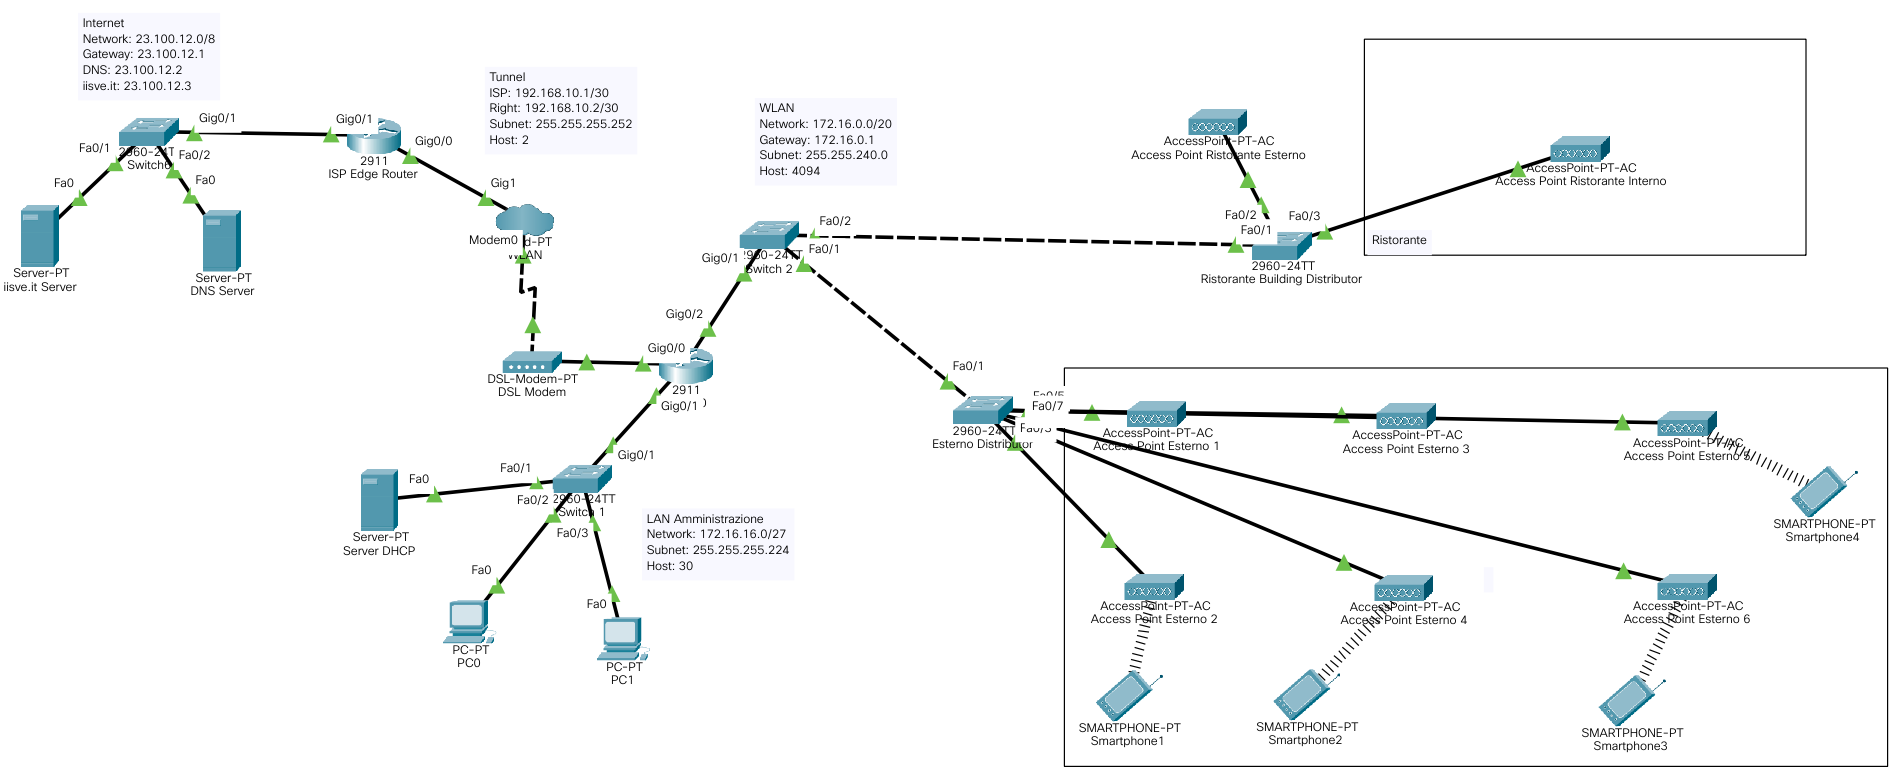
\includegraphics[width=\linewidth]{rete.png}
\end{landscape}

\subsection{Firewall}
Siccome la rete ospita utenti pubblici \`e necessario limitare il traffico originato dalla rete WAN\@.

Per limitare alcune tipologie di comunicazioni \`e possibile utilizzare le Extended Access Control List (E-ACL), queste definiscono delle regole che stabiliscono che pacchetti accettare e quali rifiutare.

In questa rete sono presenti tre ACL diverse. La prima \`e un'ACL semplice, stabilisce chi pu\`o utilizzare il servizio NAT\@. In questo caso ho specificato tutti gli indirizzi privati perch\`e chiunque si connetta alla rete deve potersi interfacciare con Internet (Access List~\ref{acl:1}).

\begin{cmds}[inside]{NAT Source list}{acl:1}{Permette di utilizzare il NAT/PAT a tutti gli indirizzi privati}
    \$ access-list 1 permit 192.168.0.0 0.0.255.255\\
    \$ access-list 1 permit 172.16.0.0 0.15.255.255\\
    \$ access-list 1 deny any
\end{cmds}

La seconda ACL impedisce a pacchetti privati di uscire dalla rete, \`e necessaria perch\`e per permettere alla rete di comunicare con Internet viene impostata una route statica verso l'ISP che comprende tutti gli indirizzi IP (0.0.0.0/0). Quando un pacchetto non ha una destinazione all'interno della rete privata viene applicata la route statica verso l'ISP e se l'indirizzo IP esiste su Internet allora viene ricevuto, altrimenti viene perso nel tragitto. Una richiesta inviata ad un indirizzo IP privato non esistente verrebbe erroneamente inoltrata all'ISP contribuendo al congestionamento della connessione e causando una fuga di dati. 

\begin{cmds}[out]{GigabitEthernet0/0}{acl:2}{Filtra le comunicazioni verso indirizzi privati}
    \$ access-list 101 deny ip any 192.168.0.0 0.0.255.255\\
    \$ access-list 101 deny ip any 172.16.0.0 0.15.255.255\\
    \$ access-list 101 permit ip any any
\end{cmds}

L'ultima ACL si occupa di filtrare il traffico originato dalla rete Wi-Fi pubblica. Vengono autorizzate solo richieste DHCP all'interno della rete privata e vengono autorizzate richieste HTTP e DNS verso la rete pubblica.

\begin{cmds}[in]{GigabitEthernet0/1}{acl:3}{Filtri avanzati per traffico in uscita dal Wi-Fi pubblico}
    \$ access-list 100 permit udp any any eq 67\\
    \$ access-list 100 deny ip any 172.16.0.0 0.15.255.255\\
    \$ access-list 100 permit tcp any any eq 80\\
    \$ access-list 100 permit udp any any eq 53\\
    \$ access-list 100 deny ip any any
\end{cmds}

L'ordine di inserimento delle ACL \`e importante. La prima regola inserita \`e quella con valore maggiore, se guardiamo l'Access List~\ref{acl:3} ho prima permesso le richieste DHCP e poi ho bloccato tutte le richieste verso la rete privata. La prima regola diventa un'eccezione all'interno della seconda regola. Inoltre nel comando ``ip access-group <acl> [in/out]'' il parametro `in/out' \`e in riferimento al router. Quindi bisogna specificare `in' quando il traffico \`e in arrivo verso il Router e `out' viceversa.

\setlength{\parskip}{0em}

\section{Rete completa e Codice sorgente}

Il file di Packet Tracer \`e disponibile per essere scaricato insieme al codice sorgente di questo documento nella repository di GitHub disponibile all'indirizzo \url{https://github.com/novelhawk/elaborato}.
